\documentclass[12pt,a4paper]{article}
\usepackage[utf8]{inputenc}
\usepackage{amsmath}
\usepackage{amsfonts}
\usepackage{graphicx}
\usepackage{float}
\usepackage{amssymb}
\author{Darián}
\title{Moogle Presentacion}
\begin{document}
\section{Introducción}
Moogle es una aplicación en csharp que utiliza diccionarios y búsquedas avanzadas para encontrar información específica en documentos de texto . En esta presentación , le mostrare cómo funciona MOOGLE y cómo puede ser útil para aquellos que necesitan buscar información precisa y rápida en documentos de texto .
\section{¿Cómo funciona Moogle?}
Moogle utiliza dos diccionarios : una para almacenar las palabras del documento y su puntuación , y otro para guardar el indice de cada palabra . La aplicación se divide en varias clases , incluyendo una para buscar elementos , otra para los resultados de búsqueda , un corrector de palabras , unna impletación de TF-IDF y una validación de búsqueda .   
\begin{figure}[H]
\centering
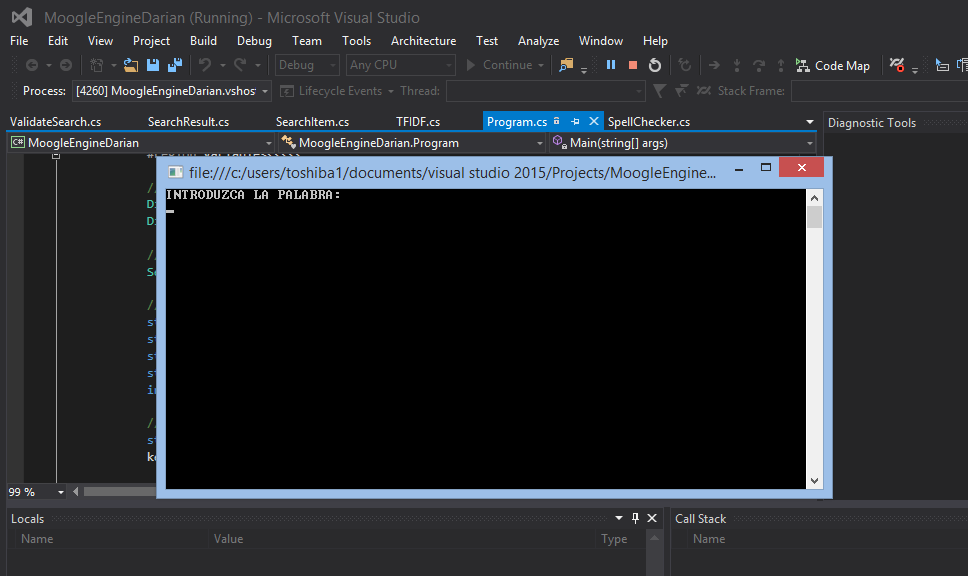
\includegraphics[scale=0.5]{Busqueda1}
\end{figure}
\begin{figure}[H]
\centering
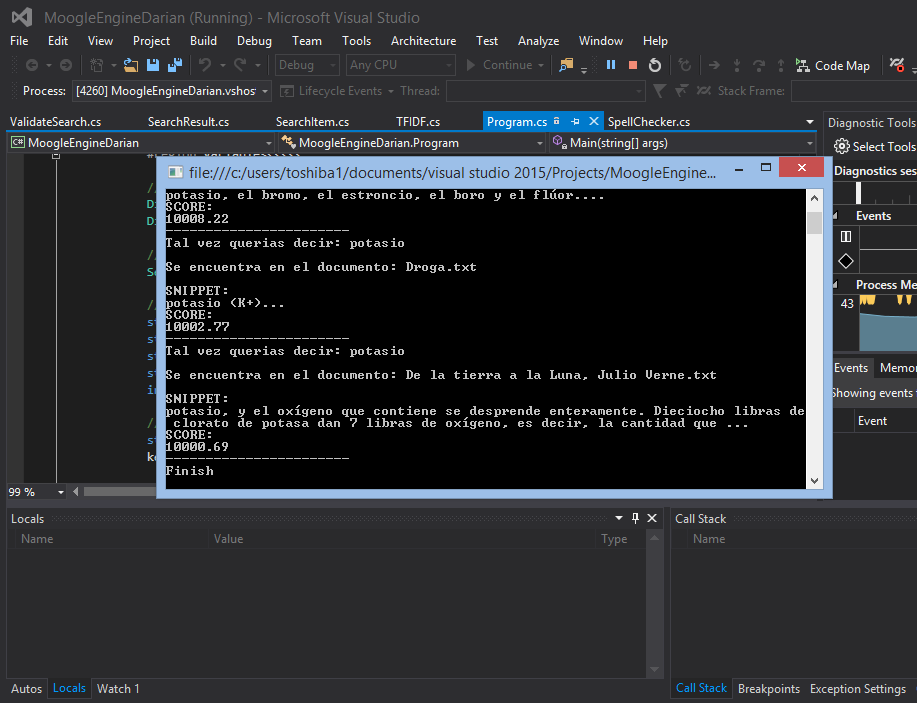
\includegraphics[scale=0.5]{Busqueda2}
\end{figure}
\section{El corrector de palabras}
Una de las caracteristicas clave de Moogle es su corrector de palabras , que ayuda a los usuarios a encontrar información incluso si no conocen la ortografía exacta de la palabra que están buscado . El corrector utiliza una comparación de letras para identificar palabras similares y sugerir posibles resultados de búsqueda . Esto se logra a través de una clase SpellChecker que compara cada palabra en el diccionario con la palabra ingresada por el usuario . Si la palabra no se encuentra en el texto , el corrector busca palabras similares y sugiere las mejores opciones de búsqueda . 
\begin{figure}[H]
\centering
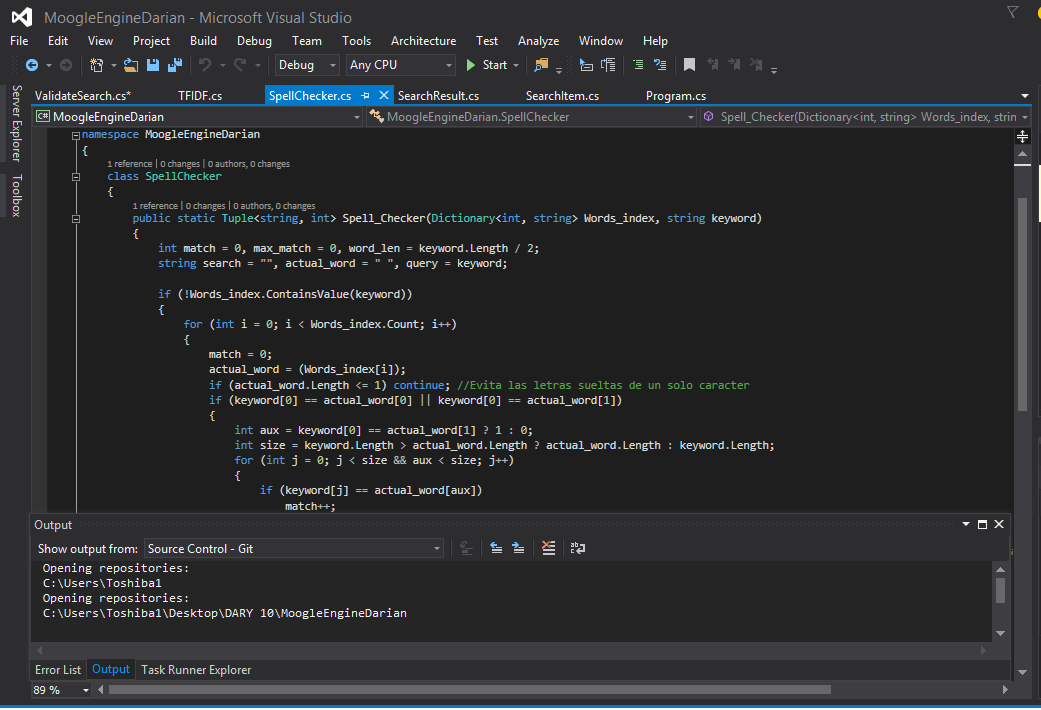
\includegraphics[scale=0.5]{SpellChecker1}
\end{figure}
\begin{figure}[H]
\centering
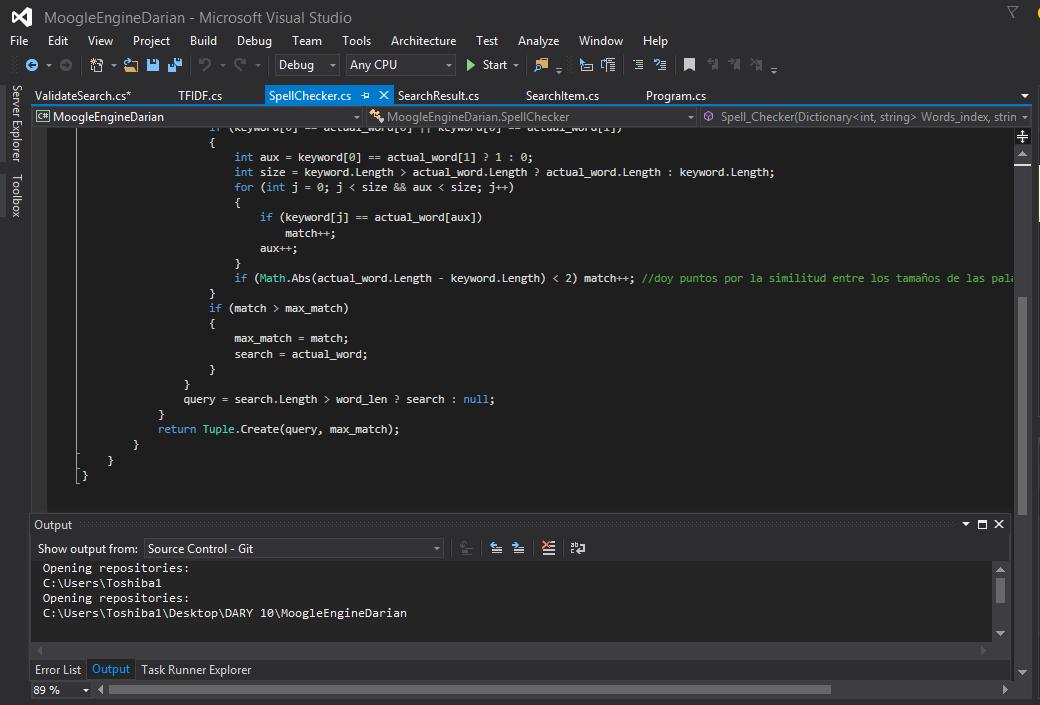
\includegraphics[scale=0.5]{SpellChecker2}
\end{figure}
\section{TF-IDF}     
Moogle también implementada TF-IDF , una técnica de procesamiento de lenguaje natural que ayuda a identificar la relavancia de una palabra en un documento específico . La puntuación  TF-IDF se utiliza para determinar qué documentos son los mas relevantes para los términos de búsqueda del usuario . La implementación de TF-IDF en Moogle se basa en el número de veces que aparece una palabra en un documento y en la frecuencia de esa palabra en todos los documentos . De esta manera , las palabras que son más comunes en un documento específico recibirán una puntuación más alta . 
\begin{figure}[H]
\centering
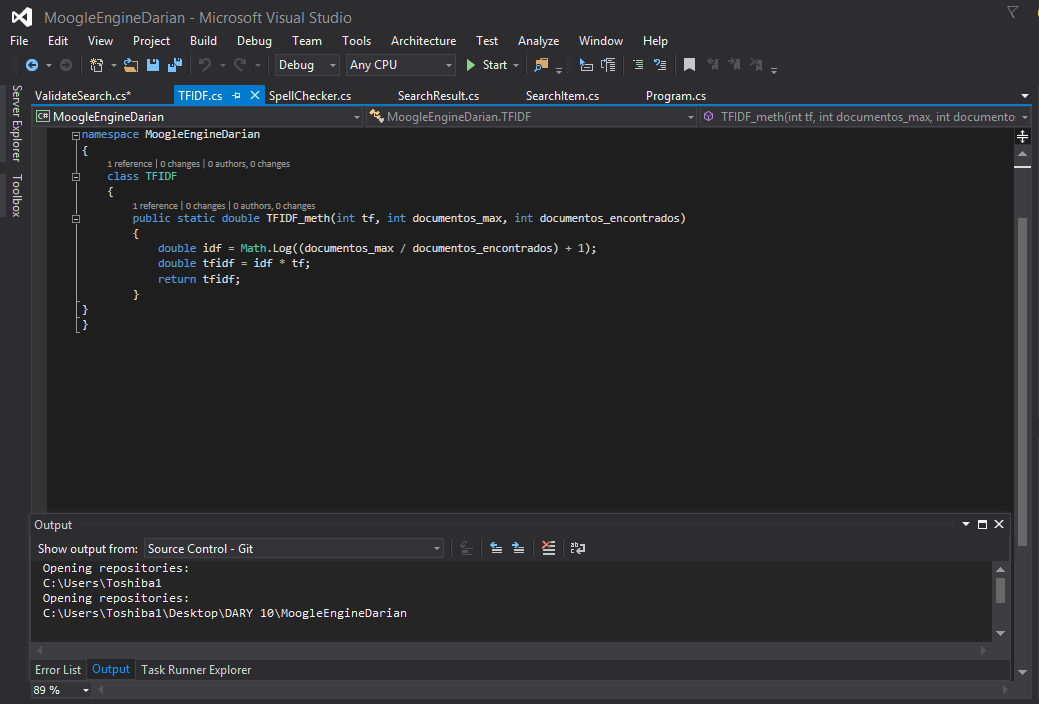
\includegraphics[scale=0.5]{TFIDF}
\end{figure}
\section{Funcionamiento de la búsqueda }
Para buscar en los documentos de texto , Moogle válida la búsqueda del usuario para asegurarse de que se ingresen al menos tres caracteres . Luego , la aplicación busca la palabra en los documentos de texto y devuelve los resultados en orden descendente según su puntuación TF-IDF . Los reultados de la búsqueda incluyen el titulo de documento , un fragmento de la oración que contiene la palabra y la puntuación TF-IDF . Además , Moogle también incluye una sugerencia de búsqueda si la palabra ingresada no se encuentra en los documenos de texto.   
\section{Conclusion}
Moogle es una herramiento útil para aquellos que necesitan buscar información específica en documentos de texto . La combinación de diccionarios , corrector de palabras y TF-IDF hace que la búsqueda sea más precisa y eficiente . Además , Moogle es fácil de usar y puede ser útil para una variedad de aplicaciones  , desde la investigación académica hasta la búsqueda de información en la industria .              
\end{document}